\documentclass[12pt]{report}

\usepackage{amssymb, fullpage, amsmath, esint}
\usepackage{graphicx}

\newtheorem{problem}{Problem}

\newenvironment{solution}[1][\it{Solution}]{\textbf{#1. } }{$\square$}

\graphicspath{ {./} }

\allowdisplaybreaks

\pagestyle{empty}

\def\Z{{\mathbb Z}}
\def\Q{{\mathbb Q}}
\def\C{{\mathbb C}}
\def\R{{\mathbb R}}
\def\N{{\mathbb N}}
\def\eps{{\epsilon}}
\def\O{{\mathcal{O}}}
\def\F{{\mathcal{F}}}
\newcommand{\floor}[1]{{\left\lfloor#1\right\rfloor}} % Floor function
\newcommand{\ceil}[1]{{\left\lceil#1\right\rceil}} % Ceiling function
\newcommand{\paren}[1]{{\left(#1\right)}} % Parentheses ()
\newcommand{\brac}[1]{{\left\{#1\right\}}} % Curly braces {}
\newcommand{\braces}[1]{{\left[#1\right]}} % Braces []
\newcommand{\abrac}[1]{{\left\langle#1\right\rangle}} % Angle Braces <>
\newcommand{\abs}[1]{{\left|#1\right|}} % Absolute value
\newcommand{\norm}[1]{{\left\|#1\right\|}} % Norm
\newcommand{\eval}[2]{\right|_{#1}^{#2}} % Evaluate

\newcommand{\pp}[2]{\frac{\partial #1}{\partial #2}} % Partial of 1 wrt 2
\newcommand{\ppn}[3]{\frac{\partial^{#1} #2}{\partial #3^{#1}}} % nth Partial of 1 wrt 2
\newcommand{\dd}[2]{\frac{\mathrm{d} #1}{\mathrm{d} #2}} % Partial of 1 wrt 2
\newcommand{\ddn}[3]{\frac{\mathrm{d}^{#1} #2}{\mathrm{d} #3^{#1}}} % nth Partial of 1 wrt 2

\def\ointcc{{\ointctrclockwise}} %counter clockwise contour integral
\def\ointc{{\ointclockwise}} %clockwise contour integral

%dash integral 
\def\Xint#1{\mathchoice
   {\XXint\displaystyle\textstyle{#1}}%
   {\XXint\textstyle\scriptstyle{#1}}%
   {\XXint\scriptstyle\scriptscriptstyle{#1}}%
   {\XXint\scriptscriptstyle\scriptscriptstyle{#1}}%
   \!\int}
\def\XXint#1#2#3{{\setbox0=\hbox{$#1{#2#3}{\int}$}
     \vcenter{\hbox{$#2#3$}}\kern-.5\wd0}}
\def\ddashint{\Xint=}
\def\dashint{\Xint-}


\begin{document}

\large

\begin{center}
 Math 567 Homework 5\\
 By Marvyn Bailly\\
\end{center}

\normalsize

\hrule

%---------------%
%---Problem 1---%
%---------------%

%--status--$

\begin{problem}
    Evaluate the integrals
    \[\frac{1}{2\pi i} \oint_C f(z) dz\] 
    where $C$ is the unit circle centered at the origin with $f(z)$ given below. Do these problems by both
    \begin{enumerate}
        \item [(i)] enclosing the singular points inside $C$
        \item [(ii)] enclosing the singular points outside $C$ (by including the point at infinity).
    \end{enumerate}
    Show that you obtain the same result in both cases.
    \begin{enumerate}
        \item [(a)] $\frac{z^2 + 1}{z^2 - a^2}, a^2 < 1$.
        \item [(b)] $\frac{z^2 + 1}{z^3}.$
        \item [(c)] $z^2e^{-1/z}$.
    \end{enumerate}
\end{problem}

\begin{solution}
    \noindent
    \begin{enumerate}
        \item [(a)]
        Consider the integral
        \[
            I = \frac{1}{2\pi i} \ointcc_C f(z) dz= \frac{1}{2\pi i} \ointcc_C \frac{z^2 + 1}{z^2 - a^2} dz,
        \]
        where $C$ is the unit circle centered at the origin and $a^2 < 1$. 
        
        \noindent
        (i) Observe that $f(z)$ has two simple poles at $\pm a$ and since $a^2 < 1$ they are within the $C$. Then by Residue theorem we have
        \[ 
            I = \text{Res}(-a) + \text{Res}(a) = \frac{(-a)^2 + 1}{-2a} + \frac{(a)^2 + 1}{2a} = 0.
        \]
        
        \noindent
        (ii) Another way to approach the problem is to consider
        \[ I = - \frac{1}{2\pi i} \ointc_C f(z) dz  =  \frac{1}{2\pi i} \ointc_C \frac{1}{t^2}f\paren{\frac{1}{t}}dt,\]
        using the transformation $z = \frac{1}{t}$ and $dz = \frac{1}{t^2}dt$. 
        We know that
        \[ \frac{1}{t^2}f\paren{\frac{1}{t}}  = \frac{1}{t^2} \cdot \frac{1 + t^2}{1 - a^2t^2},\]
        which has a double pole at $t = 0$. Applying the Residue theorem we have
        \begin{align*}
            I &= \lim_{t \to 0} \frac{d}{dt} \paren{\frac{1 + t^2}{1 - a^2t^2}}\\
            &= \lim_{t \to 0} \frac{(1 - a^2t^2)2t + (1 + t^2)2a^2t}{(1 - a^2t^2)^2}\\
            &= \lim_{t \to 0} \frac{t(2 + 2a^2)}{(1 - a^2t^2)^2}\\
            &= 0.
        \end{align*} 
        Thus we have that 
        \[ I = - \frac{1}{2\pi i} \ointc_C f(z) dz = 0.\]
        \item [(b)]
        Consider the integral
        \[ I = \frac{1}{2\pi i} \ointcc_C f(z) dz = \frac{1}{2\pi i} \ointcc_C \frac{z^2 + 1}{z^3} dz.\]
        
        \noindent
        (i)
        Notice that there is a triple pole at $z = 0$ which is within $C$. Now let's find the residue at this point,
        \begin{align*}
            \text{Res}(0) &= \frac{1}{2} \lim_{z \to 0} \ddn{2}{}{z}\paren{\frac{z^2+1}{z^3}}\paren{z^3}\\
            &= \frac{1}{2}\lim_{z \to 0} \ddn{2}{}{z} \paren(z^2 + 1)\\
            &= 1.
        \end{align*}
        Thus by the residue theorem,
        $I = 1$.

        \noindent
        (ii) Alternatively we can apply the transformation $z = \frac{1}{t}$ and $dz = \frac{1}{t^2}dt$,
        \[ I = -\frac{1}{2\pi i} \ointc_C f(z) dz = \frac{1}{2\pi i} \ointc_C \frac{1}{t^2}f\paren{\frac{1}{t}}. \]
        Notice that
        \[ \frac{1}{t^2}f\paren{\frac{1}{t}} = \frac{1}{t^2}(t + t^3) = t + \frac{1}{t},\]
        which has a simple pole at $t = 0$. Now let's find the residue at this point
        \begin{align*}
            \text{Res}(0) &= \lim_{t \to 0}(t)(\frac{1}{t} + t)\\
            &= \lim_{t \to 0} (1 + t^2)\\
            &= 1.
        \end{align*}
        Thus by the Residue Theorem we have that
        \[ I = 1.\]
        \item [(c)]
        Consider the integral
        \[ 
            I = \frac{1}{2\pi i} \ointcc_C (z^2e^{-1/z})dz = \frac{1}{2\pi i} \ointcc_C z^2(1 - \frac{1}{z} + \frac{1}{2z^2} - \frac{1}{6z^3} + \cdots)dz,
        \]
        and let
        \[ f(z) = z^2e^{-1/z}.\]
        \noindent
        (i) Notice that the integral has a pole at $z = 0$, we can find the residue by noting that the Taylor expansion of $f(z)$,
        \[ f(z) = z^2 - z + \frac{1}{2} - \frac{1}{6z} + \cdots .\]
        Thus by the definition of residue, we know that $\text{Res}(0) = - \frac{1}{6}.$ Therefore by the Residue Theorem we have found that
        \[ I = - \frac{1}{6}.\] 

        \noindent
        (ii)
        Alternatively consider the transformation $z = \frac{1}{t}$ and $dt = - \frac{1}{t^2}dt$,
        \[ I = -\frac{1}{2\pi i} \ointc_C f(z) dz = \frac{1}{2\pi i} \ointc_C \frac{1}{t^2}f\paren{\frac{1}{t}}. \]
        Then we have that,
        \[ \frac{1}{t^2}f\paren{\frac{1}{t}} = \frac{1}{t^4}(1 - t + \frac{t^2}{2} - \frac{t^3}{6} + \cdots ) = \frac{1}{t^4} - \frac{1}{t^3} + \frac{1}{2t^2} - \frac{1}{6t} + \cdots.\]
        Once again we have a simple pole at $t = 0$ which we know has residue $- \frac{1}{6}.$ Thus by the residue theorem we know that
        \[ I = - \frac{1}{6}.\]

    \end{enumerate}
\end{solution}

%----------------------------------------------------------------------------------------------------%
%\vskip 20pt
\newpage

%---------------%
%---Problem 2---%
%---------------%

%--status--$

\begin{problem}
    Find the Fourier transformation of
    \[ 
    f(t) = 
    \begin{cases}
        1 & \text{for} ~ -a < t < a\\
        0 & \text{otherwise}
    \end{cases}.
    \]
    Then, do the inverse transform using techniques of contour integration.
\end{problem}

\begin{solution}
    \noindent
    Consider the function
    \[ 
        f(t) = 
        \begin{cases}
            1 & \text{for} ~ -a < t < a\\
            0 & \text{otherwise}
        \end{cases}.
    \]
    We wish to take the Fourier transformation of $f(t)$ and then apply the inverse. First let's take the Fourier transformation of $f(t)$
    \begin{align*}
        \F[f(t)] &= F(\lambda)\\
        &= \int_{-\infty}^{\infty}f(t)e^{i\lambda t}dt\\
        &= \int_{-a}^{a} e^{i\lambda t}dt\\
        &= \frac{1}{\lambda i}\left[ e^{i\lambda t}\right]^a_{-a}\\
        &= \frac{1}{\lambda i}\paren{e^{i\lambda a} - e^{-i \lambda a}}\\
        &= \frac{2}{\lambda}\sin(\lambda a). 
    \end{align*}
    Thus we have that
    \[ \F[f(t)] = F(\lambda) = \frac{2}{\lambda}\sin(\lambda a).\]
    Next we wish to take the inverse Fourier transformation of $F(\lambda)$ which is given by
    \[\F^{-1}[F(\lambda)] = f(t) = \frac{1}{2\pi}\int_{-\infty}^{\infty}e^{-i\lambda t} \frac{2}{\lambda}\sin(\lambda a)d\lambda.\]
    We note that this integral is proper and thus we have that
    \begin{align*}
        f(t) &= \frac{1}{2\pi}\int_{-\infty}^{\infty}e^{-i\lambda t} \frac{2}{\lambda}\sin(\lambda a)d\lambda\\
        &=\frac{1}{2\pi}\dashint_{-\infty}^{\infty}e^{-i\lambda t} \frac{2}{\lambda}\sin(\lambda a)d\lambda\\
        &=\frac{1}{2\pi}\dashint_{-\infty}^{\infty}e^{-i\lambda t} \frac{e^{i\lambda a} - e^{-i \lambda a}}{\lambda} d\lambda\\
        &=\frac{1}{2\pi}\dashint_{-\infty}^{\infty} \frac{e^{i\lambda (a - t)} - e^{-i \lambda (a + t)}}{\lambda} d\lambda\\.
    \end{align*}
    Now if we define 
    \[ I(y) = \frac{1}{2\pi i} \dashint_{-\infty}^{\infty} \frac{e^{i\lambda y}}{\lambda} d\lambda\]
    we can rewrite $\F^{-1}$ as
    \[ \F^{-1}[F(\lambda)] = I(a -t) - I(-(a+t)).\]
    This gives us three cases to consider, when $y=0, y < 0,$ and $y > 0$.

    \noindent
    First let's consider when $y =0$. This gives that
    \begin{align*}
        I(y) &= \frac{1}{2\pi i} \dashint_{-\infty}^{\infty} \frac{e^{i\lambda 0}}{\lambda} d\lambda\\
        &= \frac{1}{2\pi i} \dashint_{-\infty}^{\infty} \frac{1}{\lambda} d\lambda\\
        &= \frac{1}{2\pi i} \left[ \frac{-1}{\lambda^2}\right]^\infty_{-\infty}\\
        &= 0.
    \end{align*}

    \noindent
    Next let's consider when $y > 0$. Let's form the contour shown in the following image (kindly drawn by Rohin Gilman)
    
    \begin{center}
        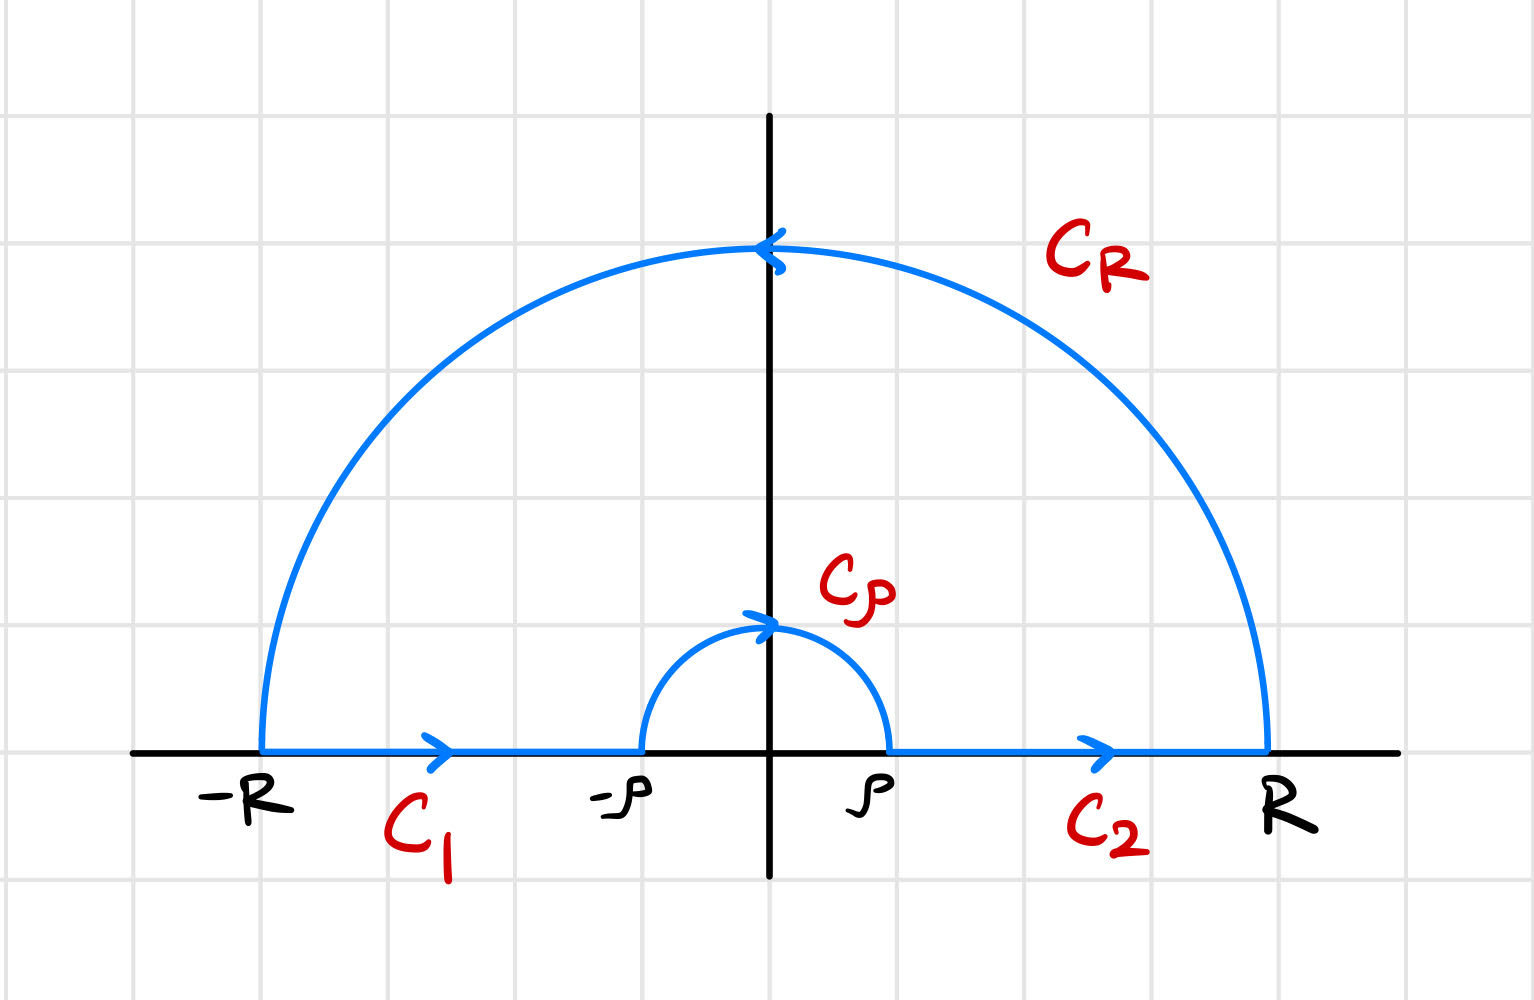
\includegraphics[width=.6\textwidth]{figures/2a.jpg}
    \end{center}

    where $C = C_1 + C_\rho + C_2 + C_R$. Note that $\frac{e^{i \lambda y}}{\lambda}$ is analytic inside and on $C$ and thus by Cauchy's Theorem we have that
    \[ \frac{1}{2\pi i} \ointcc_{C} \frac{e^{i\lambda y}}{\lambda} d\lambda = 0.\]
    For $C_R$ we have that
    \[ \abs{\frac{1}{\lambda}} \to 0 ~~\text{as}~~ \abs{\lambda} \to \infty,\]
    and thus by Jordan's Lemma
    \[\lim_{R \to \infty} \frac{1}{2\pi i} \int_{C_R} \frac{e^{i\lambda y}}{\lambda} d\lambda = 0.\]
    Next let's consider $C_\rho$ which has a simple pole at $\lambda = 0$ which is within $C_\rho$. We can compute the residue to be
    \begin{align*}
        \text{Res}(0) &= \lim_{\lambda \to 0}\frac{\lambda e^{i\lambda y}}{\lambda}\\
        &= \lim_{\lambda \to 0}e^{i\lambda y}\\
        &= e^0\\
        &= 1.
    \end{align*}
    Thus by Residue theorem we have that
    \[
        \frac{1}{2\pi i} \int_{C_R} \frac{e^{i\lambda y}}{\lambda} d\lambda = \frac{1}{2\pi i}(-i \pi)(1) = - \frac{1}{2}.
    \]
    Next let's look at $C_1$ and $C_2$, observe that
    \[ \frac{1}{2\pi i}\paren{\int_{C_1} + \int_{C_2}}\frac{e^{i \lambda y}}{\lambda}d\lambda = \frac{1}{2\pi i}\dashint_{-\infty}^{\infty}\frac{e^{i \lambda y}}{\lambda}d\lambda = I(y).\]
    Now if we collect all our terms we see that
    \[\frac{1}{2\pi i} \ointcc_{C} \frac{e^{i\lambda y}}{\lambda} d\lambda = I(y) - \frac{1}{2}  = 0,\]
    and thus 
    \[ I(y) = \frac{1}{2}.\]

    \noindent
    Next let's consider when $y<0$. Let's form the contour shown in the following image (kindly drawn by Rohin Gilman)
    
    \begin{center}
        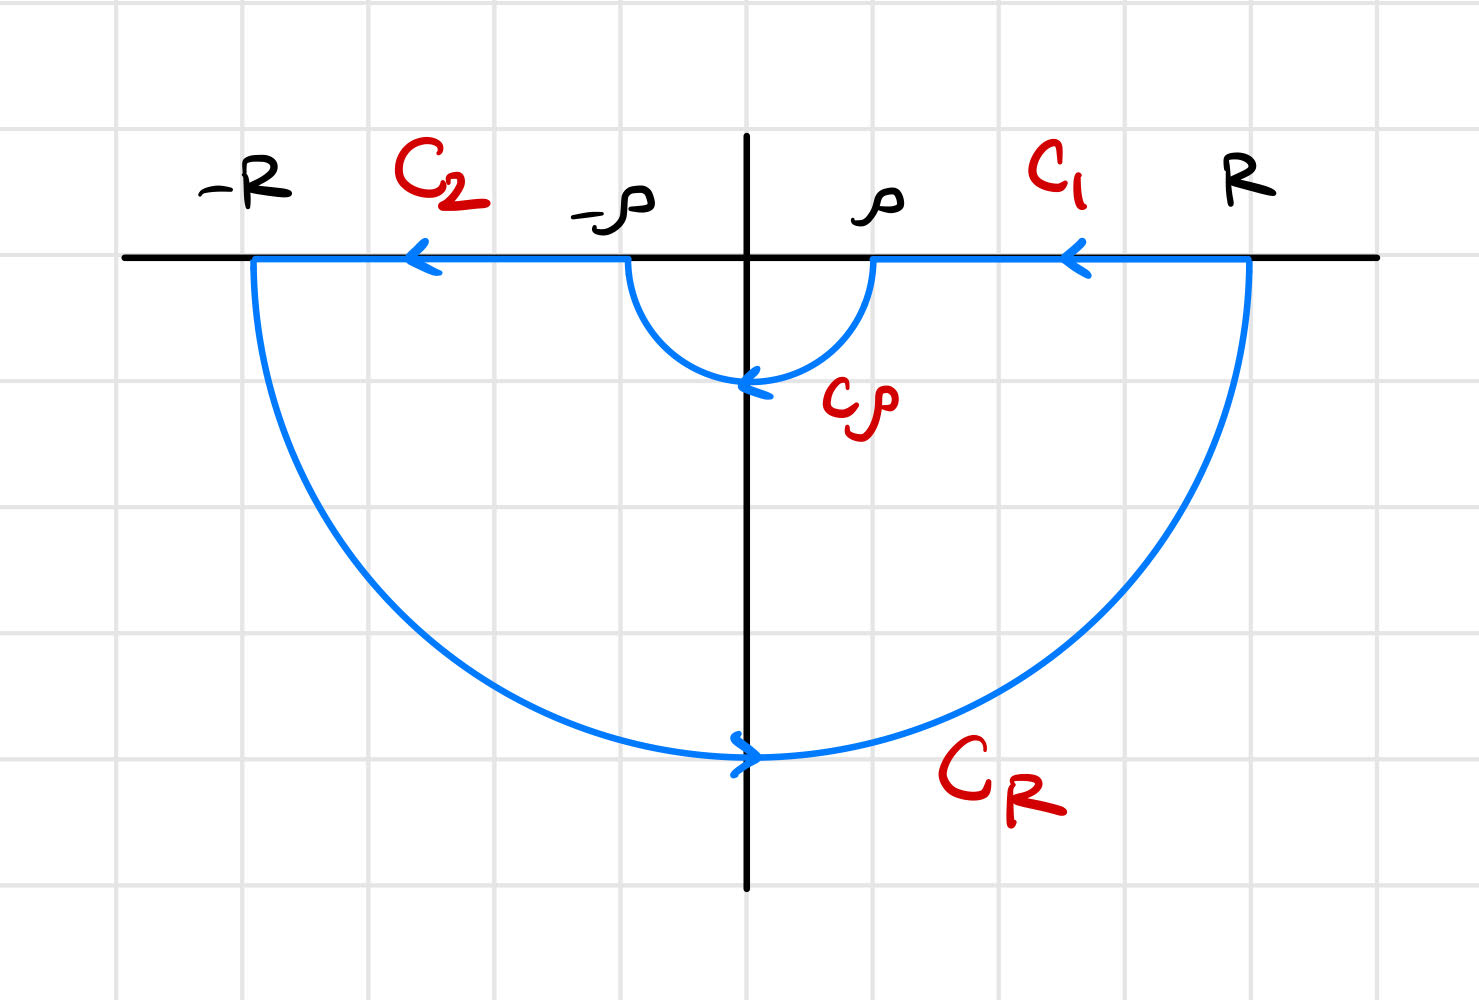
\includegraphics[width=.6\textwidth]{figures/2b.jpg}
    \end{center}

    where $C = C_1 + C_\rho + C_2 + C_R$. Note that $\frac{e^{i \lambda y}}{\lambda}$ is analytic inside and on $C$ and thus by Cauchy's Theorem we have that
    \[ \frac{1}{2\pi i} \ointcc_{C} \frac{e^{i\lambda y}}{\lambda} d\lambda = 0.\]
    For $C_R$ we have that
    \[ \abs{\frac{1}{\lambda}} \to 0 ~~\text{as}~~ \abs{\lambda} \to \infty,\]
    and thus by Jordan's Lemma
    \[\lim_{R \to \infty} \frac{1}{2\pi i} \int_{C_R} \frac{e^{i\lambda y}}{\lambda} d\lambda = 0.\]
    Next let's consider $C_\rho$ which has a simple pole at $\lambda = 0$ which is within $C_\rho$. We can compute the residue to be
    \begin{align*}
        \text{Res}(0) &= \lim_{\lambda \to 0}\frac{\lambda e^{i\lambda y}}{\lambda}\\
        &= \lim_{\lambda \to 0}e^{i\lambda y}\\
        &= e^0\\
        &= 1.
    \end{align*}
    Thus by Residue theorem we have that
    \[
        \frac{1}{2\pi i} \int_{C_R} \frac{e^{i\lambda y}}{\lambda} d\lambda = \frac{1}{2\pi i}(-i \pi)(1) = - \frac{1}{2}.
    \]
    Next let's look at $C_1$ and $C_2$, observe that
    \[ \frac{1}{2\pi i}\paren{\int_{C_1} + \int_{C_2}}\frac{e^{i \lambda y}}{\lambda}d\lambda = -\frac{1}{2\pi i}\dashint_{-\infty}^{\infty}\frac{e^{i \lambda y}}{\lambda}d\lambda = -I(y).\]
    Now if we collect all our terms we see that
    \[\frac{1}{2\pi i} \ointcc_{C} \frac{e^{i\lambda y}}{\lambda} d\lambda = -I(y) - \frac{1}{2}  = 0,\]
    and thus 
    \[ I(y) = -\frac{1}{2}.\]
    Considering all three cases of $y$ we get that $I(y) = \frac{1}{2}\text{sgn}(y)$. This means that
    \[ \F^{-1}[F(\lambda)] = \frac{1}{2}\paren{\text{sgn}(a -t) + \text{sgn}(a+t)}.\]
    This means that within the interval $-a < t < a$ we have that $\text{sgn}(a-t)=\text{a+t} = 1$ which implies that $\F^{-1} = f(t) = 1$ within the interval. Considering the end points $\pm a$ we get that,
    \begin{align*}
        f(\pm a) &= \frac{1}{2}\paren{\text{sgn}(a \mp a) + \text{sgn}(a \pm a)}\\
        &=\frac{1}{2}(1)\\
        &= \frac{1}{2}.
    \end{align*}
    Thus we have that
    \[ \F^{-1}[F(\lambda)] = 
    \begin{cases}
    1 &\text{for} ~ -a < t < a\\
    \frac{1}{2} &\text{for} ~ - t = \pm a\\
    0 &\text{otherwise}\\
    \end{cases},
    \]
    which is the expected solution. 
\end{solution}

%----------------------------------------------------------------------------------------------------%
%\vskip 20pt
\newpage

%---------------%
%---Problem 3---%
%---------------%

%--status--$

\begin{problem}
    Consider the function
    \[ f(z) = \ln(z^2 -1),\]
    made single-valued by restricting the angles in the following ways, with $z_1 = z - 1 = r_1 e^{i\theta_1}$ and $z_2 = z +1 = r_2e^{i\theta_2}$ of
    \begin{enumerate}
        \item [(a)] $-3\pi/2 < \theta_1 \leq \pi / 2, - 3\pi /2 < \theta_2 \leq \pi / 2$
        \item [(b)] $0 < \theta_1 \leq 2 \pi, 0 < \theta_2 \leq 2 \pi$
        \item [(c)] $-\pi < \theta_1 \leq \pi, 0 < \theta_2 \leq 2 \pi.$
    \end{enumerate} 
    Find where the branch cuts are for each case by locating where the function is discontinuous. Use the AB tests ad show your results. 
\end{problem}

\begin{solution}

    \noindent
    Let $f(z) = \ln(z^2 -1)$, $z_1 = z - 1 = r_1 e^{i\theta_1}$ and $z_2 = z +1 = r_2e^{i\theta_2}.$
    \begin{enumerate}
        \item [(a)]
        Consider the interval $-3\pi/2 < \theta_1 \leq \pi / 2, - 3\pi /2 < \theta_2 \leq \pi / 2$ on which $f(z)$ is single-valued. The following figure, kindly provided by Rohin Gilman, shows the branch cuts at $\pm 1 + ai$ of $f(z)$. 
        \begin{center}
            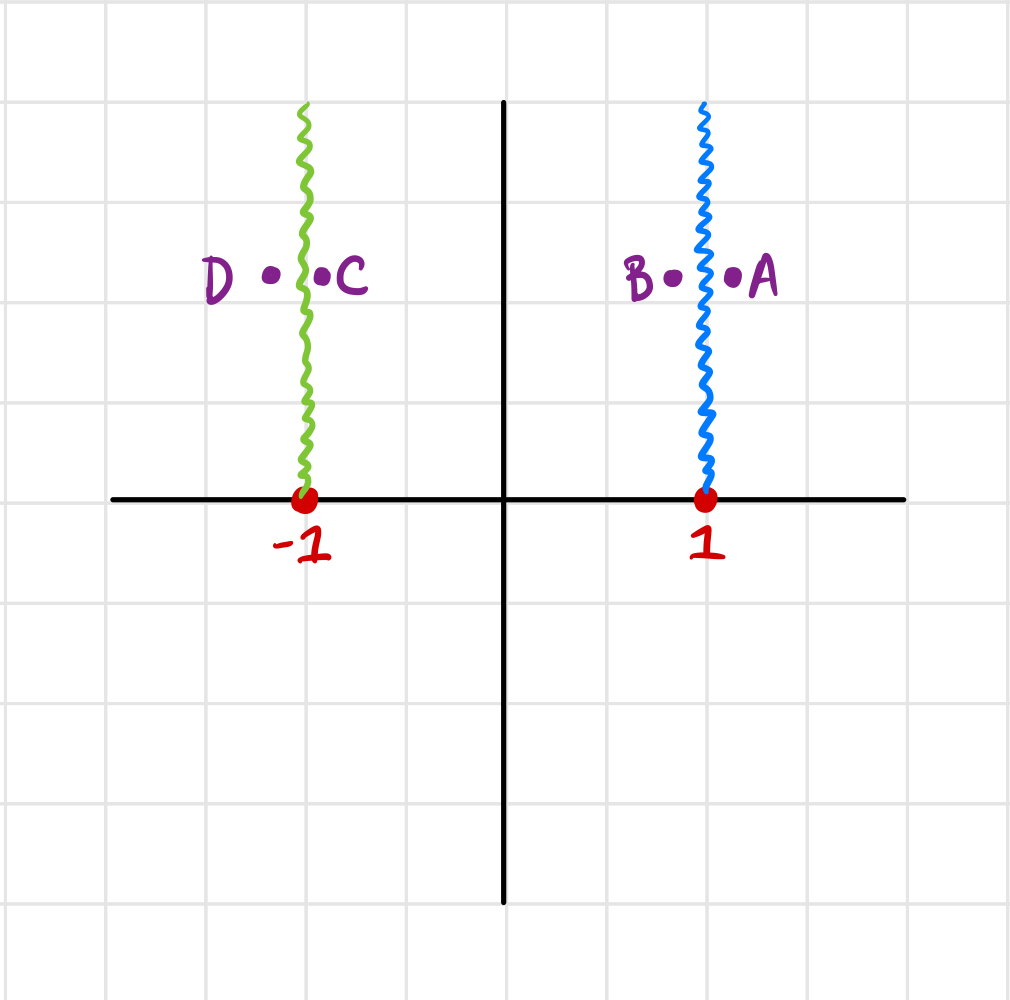
\includegraphics[width=.5\textwidth]{figures/3a.png}
        \end{center}
        Now let's consider the branch cut at $1 + ai$. At the point $A$, we can say that $\theta_1 = -\frac{3\pi}{2}$ and $\theta_2 = \arcsin\paren{\frac{r_1}{r_2}}$. Then we have that
        \begin{align*}
            \ln((z-1)(z+1)) &= \ln(r_1e^{i\theta_1}r_2e^{i\theta_2})\\
            &=\ln(r_1r_2) + i\paren{-\frac{3\pi}{2} + \arcsin\paren{\frac{r_1}{r_2}}}.
        \end{align*}
        Next consider the point $B$ on the other side of the branch cut. We can say that $\theta_1 = \frac{\pi}{2}$ and $\theta_2 = \arcsin\paren{\frac{r_1}{r_2}}$. Then we have that
        \begin{align*}
            \ln((z-1)(z+1)) &= \ln(r_1e^{i\theta_1}r_2e^{i\theta_2})\\
            &=\ln(r_1r_2) + i\paren{\frac{\pi}{2} + \arcsin\paren{\frac{r_1}{r_2}}}.
        \end{align*}
        Since the values at points $A$ and $B$ are not equal, we know that $f$ is discontinuous along $1 + ai$ and thus the branch cut does not cancel and remains. Next let's consider the branch cut along $-1 + ai$. First let's look at the point $C$. If we let $\theta_1 = \arcsin\paren{\frac{r_2}{r_1}} - \pi$ and $\theta_2 = -\frac{3\pi}{2}$. From this we get
        \begin{align*}
            \ln((z-1)(z+1)) &= \ln(r_1e^{i\theta_1}r_2e^{i\theta_2})\\
            &=\ln(r_1r_2) + i\paren{\arcsin\paren{\frac{r_2}{r_1}} - \pi - \frac{3\pi}{2}}.
        \end{align*}
        Next consider the point $D$, if we let $\theta_1 = \arcsin\paren{\frac{r_2}{r_1}} - \pi$ and $\theta_2 = \frac{\pi}{2}$. From this we get
        \begin{align*}
            \ln((z-1)(z+1)) &= \ln(r_1e^{i\theta_1}r_2e^{i\theta_2})\\
            &=\ln(r_1r_2) + i\paren{\arcsin\paren{\frac{r_2}{r_1}} - \pi - \frac{\pi}{2}}.
        \end{align*}
        Since the values at $C$ and $D$ are different, we have that $f$ is discontinuous along $-1+ai$ and thus the branch cut remains.

        \item [(b)]
        Consider the interval $0 < \theta_1 \leq 2 \pi, 0 < \theta_2 \leq 2 \pi$ on which $f(z)$ is single-valued. The following figure, kindly provided by Rohin Gilman, shows the branch cuts at $1 < x < \infty$ and $-1 \leq x \leq 1$ of $f(z)$. 


        \begin{center}
            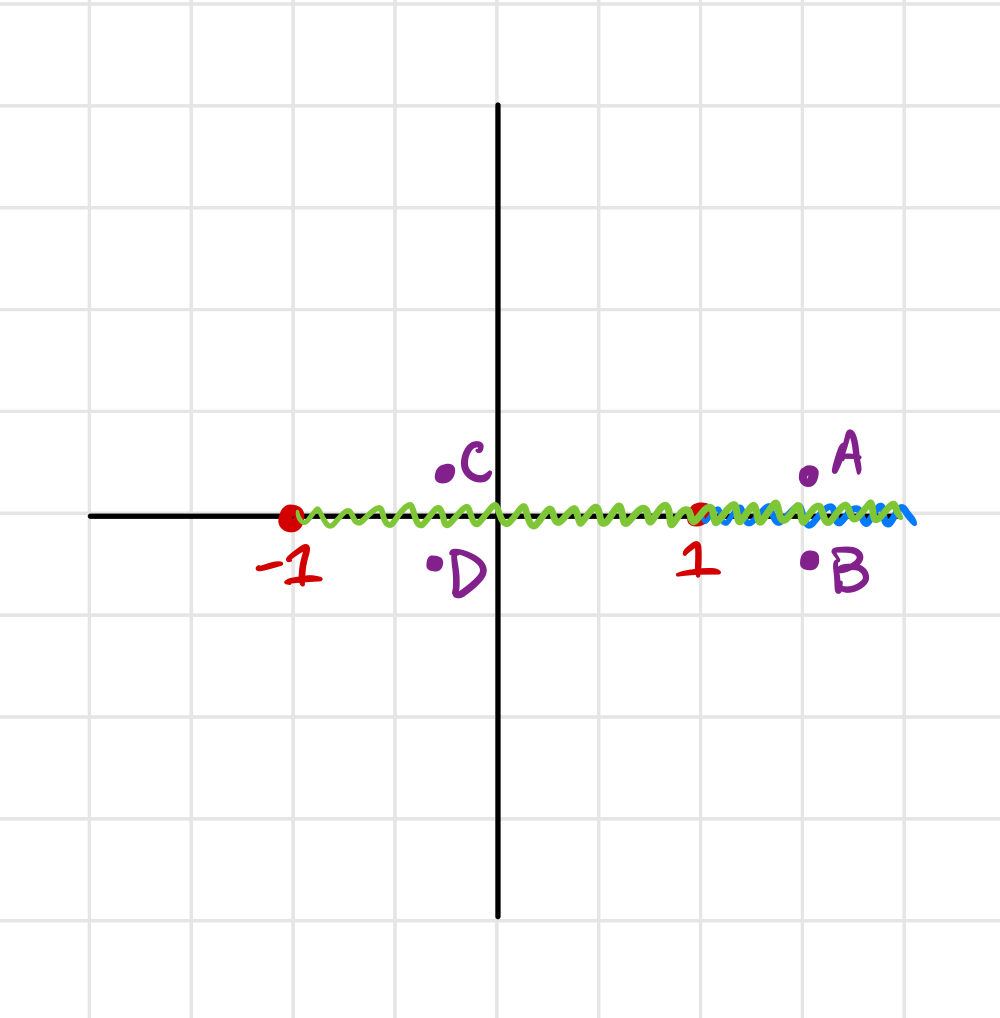
\includegraphics[width=.5\textwidth]{figures/3b.png}
        \end{center}
        
        Now let's consider the branch cut along $1 < x < \infty$. At the point $A$, we can have $\theta_1 = 0$ and $\theta_2 = 0$. This gives us that
        \begin{align*}
            \ln((z-1)(z+1)) &= \ln(r_1e^{i\theta_1}r_2e^{i\theta_2})\\
            &=\ln(r_1r_2).
        \end{align*}
        Next let's consider the point $B$, where $\theta_1 = 2\pi$ and $\theta_2 = 2\pi$. Thus we have that
        \begin{align*}
            \ln((z-1)(z+1)) &= \ln(r_1e^{i\theta_1}r_2e^{i\theta_2})\\
            &=\ln(r_1r_2) + i(4\pi).
        \end{align*}
        We can see that the values at point $A$ and $B$ are different and thus $f$ is discontinuous along the branch cut $1 < x < \infty$. Therefore the branch cut remains.  Next let's consider the branch cut $1 \leq x \leq 1$. First consider the point $C$, then $\theta_1 = \pi$ and $\theta_2 = 0$ and we have that
        \begin{align*}
            \ln((z-1)(z+1)) &= \ln(r_1e^{i\theta_1}r_2e^{i\theta_2})\\
            &=\ln(r_1r_2) + i(\pi).
        \end{align*}
        Finally consider the point $D$, where $\theta_1 = \pi$ and $\theta_2 = 2\pi$. Then we have that
        \begin{align*}
            \ln((z-1)(z+1)) &= \ln(r_1e^{i\theta_1}r_2e^{i\theta_2})\\
            &=\ln(r_1r_2) + i(3\pi).
        \end{align*}
        Since the values at $C$ and $D$ are not equal, $f$ is discontinuous along the branch cut $-1\leq x\leq 1$. Therefore the branch cut remains. 


        \item [(c)]
        Finally consider the interval $-\pi < \theta_1 \leq \pi, 0 < \theta_2 \leq 2 \pi$ on which $f$ is discontinuous along the branch cuts $-1 < x < \infty$ and $-\infty < x < 1$. The following figure, kindly provided by Rohin Gilman, shows this behavior.

        \begin{center}
            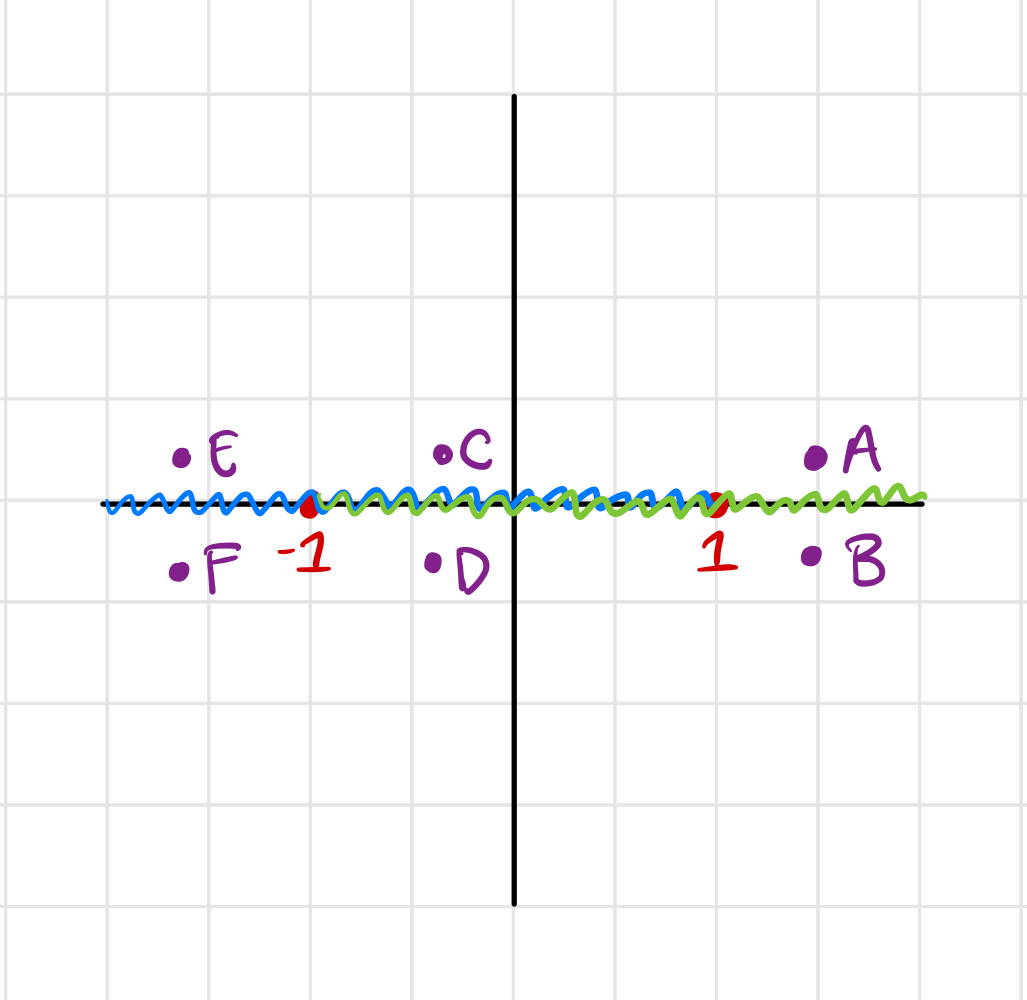
\includegraphics[width=.5\textwidth]{figures/3c.png}
        \end{center}
        
        First let's consider the points $A$ and $B$. At the point $A$, we can let $\theta_1 = 0$ and $\theta_2 = 0$. Then we have that
        \begin{align*}
            \ln((z-1)(z+1)) &= \ln(r_1e^{i\theta_1}r_2e^{i\theta_2})\\
            &=\ln(r_1r_2).
        \end{align*}
        Next consider the point $B$, where $\theta_1 = 0$ and $\theta_2 = 2\pi$. Then we have that
        \begin{align*}
            \ln((z-1)(z+1)) &= \ln(r_1e^{i\theta_1}r_2e^{i\theta_2})\\
            &=\ln(r_1r_2) + i(2\pi).
        \end{align*}
        Since the values at are not equal, we know that the $f$ is discontinuous along $1 < x < \infty$ and this section of the branch cut remains. Next let's consider the points $C$ and $D$. At $C$ we have that $\theta_1 = \pi$ and $\theta_2 = 0$ which gives that
        \begin{align*}
            \ln((z-1)(z+1)) &= \ln(r_1e^{i\theta_1}r_2e^{i\theta_2})\\
            &=\ln(r_1r_2) + i(\pi).
        \end{align*}
        Next let's consider the point $D$ then $\theta_1 = -\pi$ and $\theta_2 = 2\pi$ which gives
        \begin{align*}
            \ln((z-1)(z+1)) &= \ln(r_1e^{i\theta_1}r_2e^{i\theta_2})\\
            &=\ln(r_1r_2) + i(\pi).
        \end{align*}
        Since these values are equal, $f$ is continuous here. Thus the branch cuts going from $-1 \leq x \leq 1$ cancel each other. Finally let's consider the points $E$ and $F$. At point $E$, we say that $\theta_1 = \pi$ and $\theta_2 = \pi$. Thus we have that
        \begin{align*}
            \ln((z-1)(z+1)) &= \ln(r_1e^{i\theta_1}r_2e^{i\theta_2})\\
            &=\ln(r_1r_2) + i(2\pi).
        \end{align*}
        Next consider $F$ where $\theta_1 = -\pi$ and $\theta_2 = \pi$. From this we know that 
        \begin{align*}
            \ln((z-1)(z+1)) &= \ln(r_1e^{i\theta_1}r_2e^{i\theta_2})\\
            &=\ln(r_1r_2).
        \end{align*}
        Since these two values are different, $f$ is discontinuous along $-\infty < x < -1$ and thus the branch cut remains.

    \end{enumerate}
\end{solution}

%----------------------------------------------------------------------------------------------------%
%\vskip 20pt
\newpage
\end{document}